% generated by scripts/pkl_to_latex.py
% source PKL : uscan_v1_L6_Ne6_t0p1_mode-uniform_nmin2_solver-gcg_full_es_restarts10_iter300_kmax5_tol1em09_U0.1to5_N21-8081b758e7cc.pkl
% scan type  : uscan
% state      : ex_singlet
% requires   : \usepackage{pgfplots} \pgfplotsset{compat=1.18}
% colours match the matplotlib PDF (tab10 cycle)
\definecolor{gmeC0}{HTML}{1F77B4}
\definecolor{gmeC1}{HTML}{FF7F0E}
\definecolor{gmeC2}{HTML}{2CA02C}
\definecolor{gmeC3}{HTML}{D62728}
\definecolor{gmeC4}{HTML}{9467BD}
\definecolor{gmeC5}{HTML}{8C564B}
\definecolor{gmeC6}{HTML}{E377C2}
\definecolor{gmeC7}{HTML}{17BECF}

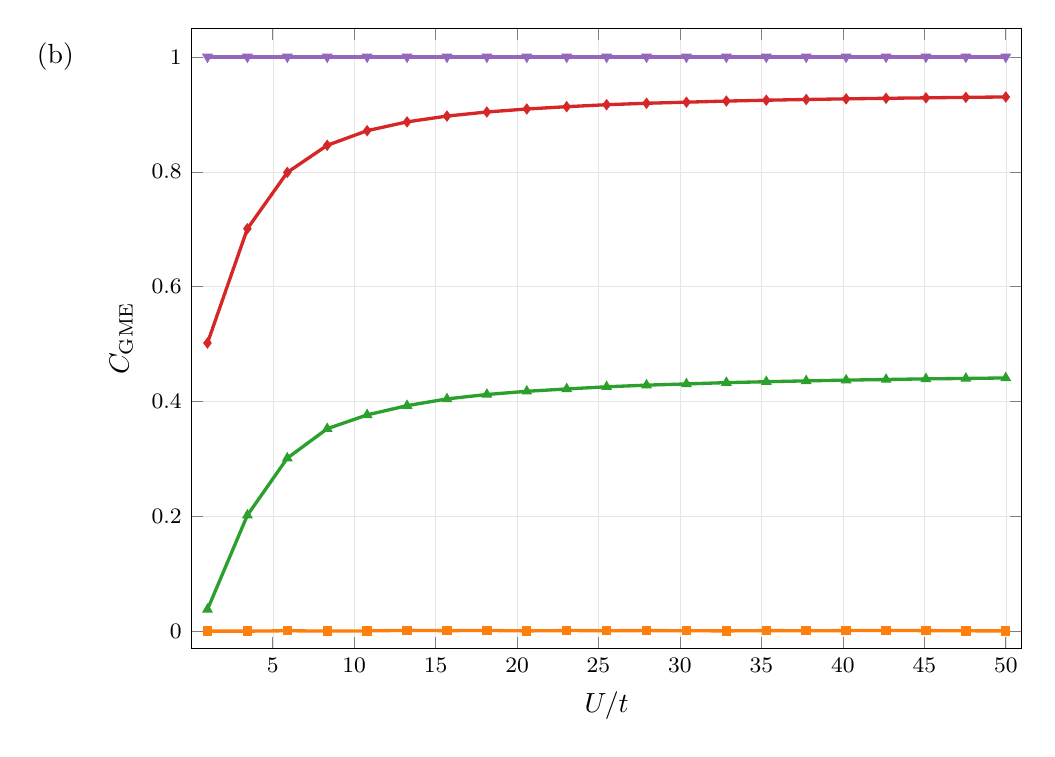
\begin{tikzpicture}
  \begin{axis}[
    width=\columnwidth,
    height=0.78\columnwidth,
    xlabel={$U/t$},
    ylabel={$C_{\mathrm{GME}}$},
    grid=both,
    grid style={line width=.1pt, draw=gray!20},
    tick label style={font=\footnotesize\rmfamily, /pgf/number format/fixed},
    label style={font=\normalsize\rmfamily},
    scaled ticks=false,
    legend style={font=\scriptsize\rmfamily, draw=gray!40, at={(0.5,1.03)}, anchor=south, /tikz/every even column/.append style={column sep=6pt}},
    legend cell align={left},
    legend columns=2,
    ymin=-0.03,
    ymax=1.05,
    xmin=0.02,
    xmax=50.98,
    after end axis/.append code={\node[anchor=east, font=\normalsize\rmfamily] at (axis description cs:-0.13,0.954) {(b)};},
  ]
    \addplot[color=gmeC1, mark=square*, mark size=1.1pt, line width=1.2pt] coordinates {
        (1,0.000076) (3.45,0.000017) (5.9,0.000725) (8.35,0.00013)
        (10.8,0.000477) (13.25,0.001416) (15.7,0.000895) (18.15,0.00125)
        (20.6,0.000461) (23.05,0.001101) (25.5,0.000825) (27.95,0.001059)
        (30.4,0.000767) (32.85,0.000458) (35.3,0.001054) (37.75,0.000683)
        (40.2,0.001019) (42.65,0.001117) (45.1,0.000989) (47.55,0.000616)
        (50,0.000467)
    };
    \addplot[color=gmeC2, mark=triangle*, mark size=1.1pt, line width=1.2pt] coordinates {
        (1,0.037744) (3.45,0.201932) (5.9,0.301295) (8.35,0.352537)
        (10.8,0.376633) (13.25,0.392703) (15.7,0.404476) (18.15,0.412167)
        (20.6,0.417721) (23.05,0.421826) (25.5,0.42556) (27.95,0.428443)
        (30.4,0.430543) (32.85,0.432829) (35.3,0.434396) (37.75,0.435873)
        (40.2,0.437172) (42.65,0.43828) (45.1,0.439383) (47.55,0.440089)
        (50,0.441003)
    };
    \addplot[color=gmeC3, mark=diamond*, mark size=1.1pt, line width=1.2pt] coordinates {
        (1,0.501818) (3.45,0.700882) (5.9,0.798874) (8.35,0.8461)
        (10.8,0.871548) (13.25,0.8869) (15.7,0.897007) (18.15,0.904106)
        (20.6,0.909344) (23.05,0.913356) (25.5,0.916801) (27.95,0.919317)
        (30.4,0.921193) (32.85,0.923135) (35.3,0.924617) (37.75,0.925893)
        (40.2,0.927003) (42.65,0.927977) (45.1,0.928743) (47.55,0.929606)
        (50,0.930293)
    };
    \addplot[color=gmeC4, mark=triangle*, mark size=1.1pt, mark options={rotate=180}, line width=1.2pt] coordinates {
        (1,1) (3.45,1) (5.9,1) (8.35,1)
        (10.8,1) (13.25,1) (15.7,1) (18.15,1)
        (20.6,1) (23.05,1) (25.5,1) (27.95,1)
        (30.4,1) (32.85,1) (35.3,1) (37.75,1)
        (40.2,1) (42.65,1) (45.1,1) (47.55,1)
        (50,1)
    };
  \end{axis}
\end{tikzpicture}
